\section{Collimator\_linear: The simple Soller blade collimator}
\label{collimator-linear}\index{Optics!Linear collimator}

\component{Collimator\_linear}{System}{$x_{min}$, $x_{max}$, $y_{min}$, $y_{max}$, $L$, $\delta$}{}{}

{\bf Collimator\_linear} models a standard linear Soller blade collimator.
The collimator has two identical rectangular openings,
defined by the $x$ and $y$ values. Neutrons not clearing both
openings are ABSORB'ed.
The length of the collimator blades is denoted $L$, while
the distance between blades is called $d$.

The collimating effect is taken care of by employing an approximately
triangular transmission through the collimator of width (FWHM) $\delta$, 
which is given in arc minutes, {\em i.e.} $\delta=60$ is one degree.
If $\delta=0$, the collimating effect is disabled,
so that the component only consists of two rectangular apertures.

For a more detailed Soller collimator simulation,
taking every blade into account, it is possible to use
{\bf Channeled\_guide} with absorbing walls, 
see section~\ref{s:channeled_guide}.

\begin{figure}[h!]
  \begin{center}
    \psfrag{xmin}[c][c]{$x_{\rm min}$}
    \psfrag{xmax}[c][c]{$x_{\rm max}$}
    \psfrag{ymin}[c][c]{$y_{\rm min}$}
    \psfrag{ymax}[c][c]{$y_{\rm max}$}
    \psfrag{delta}[c][c]{$\delta$}
    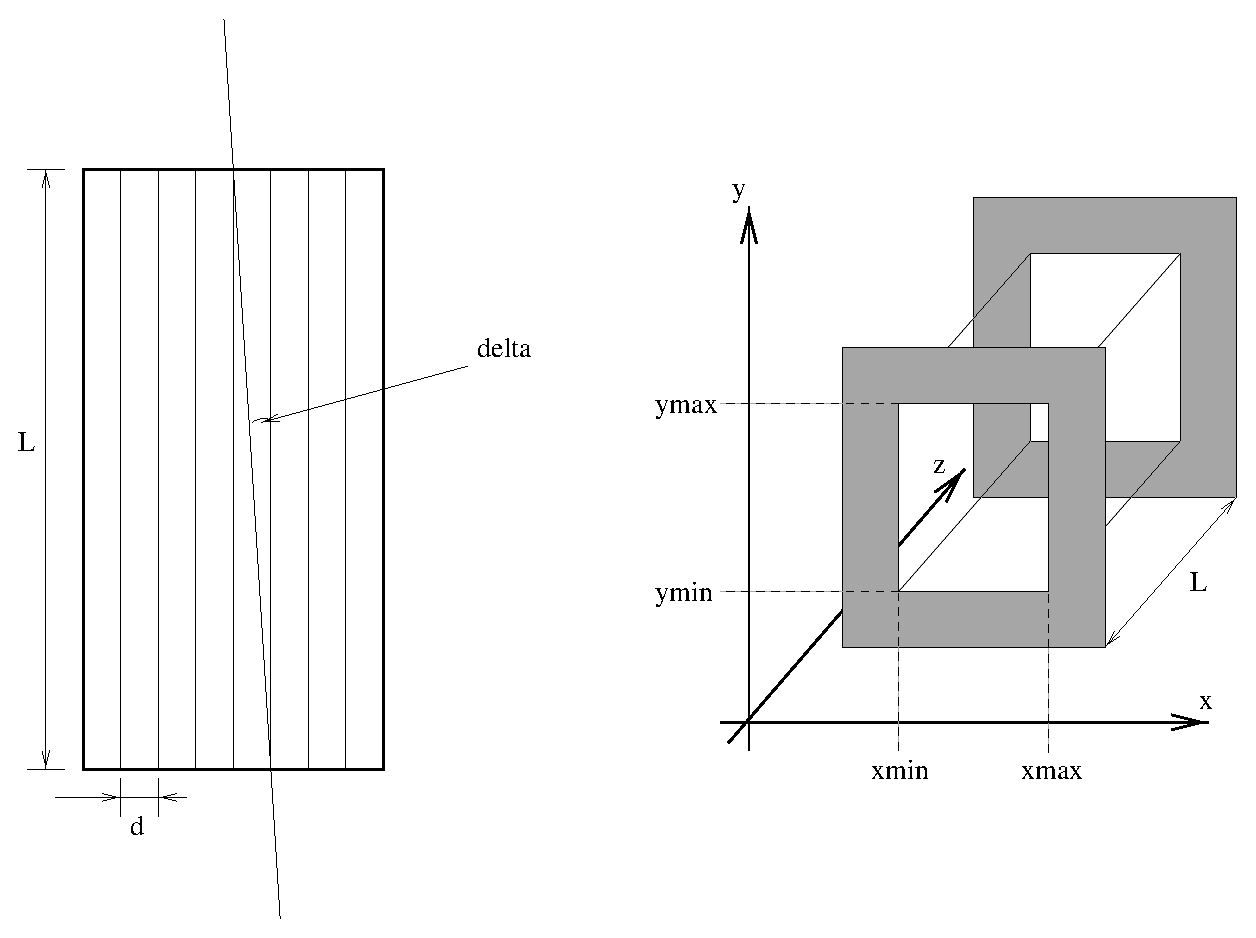
\includegraphics[width=0.7\textwidth]{figures/collimator}
  \end{center}
\caption{The geometry of a simple Soller blade collimators:
The real Soller collimator, seen from the top (left),
and a sketch of the component {\bf Soller} (right).
The symbols are defined in the text.}
\label{f:collimator}
\end{figure}

\subsection{Collimator transmission}
The horizontal divergence, $\eta_h$, is defined as the angle between the
neutron path and the vertical $y-z$ plane along the collimator axis.
We then define the collimation angle as the maximal allowed
horizontal divergence: $\delta = \tan^{-1}(d/L)$,
see Fig.~\ref{f:collimator}. Neutrons with a horizontal
divergence angle $|\eta_h| \geq \delta$ will always
hit at least one collimator blade and will thus be ABSORB'ed.
For smaller divergence angles, $|\eta_h| < \delta$, the fate of the
neutron depends on its exact entry point.
Assuming that a typical collimator has many blades, the
absolute position of each blade perpendicular to the collimator axis
is thus mostly unimportant.
A simple statistical consideration now shows that the transmission
probability is $T = 1-\tan|\eta_h|/\tan\delta$.
Often, the approximation $T \approx 1-|\eta_h|/\delta$ is used, giving
a triangular transmission profile.

\subsection{Algorithm}
The algorithm of {\rm Collimator\_linear} is roughly as follows:
\begin{enumerate}
\item Check by propagation if the neutron ray clear the entry and exit slits,
otherwise ABSORB.
\item Check if $|\eta_h| < \delta$, otherwise ABSORB.
\item Simulate the collimator transmission by a weight transformation:
\begin{equation}
\pi_i = T = 1-\tan|\eta_h|/ \tan\delta ,
\end{equation}
\end{enumerate}
